\documentclass[]{article}

% Imported Packages
%------------------------------------------------------------------------------
\usepackage{amssymb}
\usepackage{amstext}
\usepackage{amsthm}
\usepackage{amsmath}
\usepackage{enumerate}
\usepackage{fancyhdr}
\usepackage[margin=1in]{geometry}
\usepackage{graphicx}
\usepackage{multirow}
\graphicspath{ {./images/} }
%\usepackage{extarrows}
%\usepackage{setspace}
%\usepackage{xcolor}
\usepackage{color}
\usepackage{titlesec}
\usepackage{hyperref}  % Recommended for clickable links
\usepackage{url}       % If you only need URL support

%------------------------------------------------------------------------------

% Header and Footer
%------------------------------------------------------------------------------
\pagestyle{plain}  
\renewcommand\headrulewidth{0.4pt}                                      
\renewcommand\footrulewidth{0.4pt}                                    
%------------------------------------------------------------------------------

% Title Details
%------------------------------------------------------------------------------
\title{Deliverable \#1 Template : Software Requirement Specification (SRS)}
\author{SE 3A04: Software Design II -- Large System Design}
\date{}
%------------------------------------------------------------------------------

% Paragraph Formatting
%------------------------------------------------------------------------------
\setcounter{secnumdepth}{4}

\titleformat{\paragraph}
{\normalfont\normalsize\bfseries}{\theparagraph}{1em}{}
\titlespacing*{\paragraph}
{0pt}{3.25ex plus 1ex minus .2ex}{1.5ex plus .2ex}
                            
%------------------------------------------------------------------------------

% Document
%------------------------------------------------------------------------------
\begin{document}

\maketitle	
\noindent{\bf Tutorial Number:} T03\\
{\bf Group Number:} G6 \\
{\bf Group Members:} 
\begin{itemize}
	\item Cass Braun
	\item Nehad Shikh Trab
	\item Savvy Liu
	\item Tvesha Shah
	\item Victor Yu
\end{itemize}

\section*{IMPORTANT NOTES}
\begin{itemize}
	\item Be sure to include all sections of the template in your document regardless whether you have something to write for each or not
	\begin{itemize}
		\item If you do not have anything to write in a section, indicate this by the \emph{N/A}, \emph{void}, \emph{none}, etc.
	\end{itemize}
	\item Uniquely number each of your requirements for easy identification and cross-referencing
	\item Highlight terms that are defined in Section~1.3 (\textbf{Definitions, Acronyms, and Abbreviations}) with \textbf{bold}, \emph{italic} or \underline{underline}
	\item For Deliverable 1, please highlight, in some fashion, all (you may have more than one) creative and innovative features. Your creative and innovative features will generally be described in Section~2.2 (\textbf{Product Functions}), but it will depend on the type of creative or innovative features you are including.
\end{itemize}

\newpage
\section{Introduction}
\label{sec:introduction}
% Begin Section

This SRS will provide visibility over software requirements for Gaim, an AI-powered wildlife identification application. This document will discuss the purpose of Gaim, the scope of the application, its objectives, production description, any constraints, user characteristics, product requirements, and use case diagrams.


\subsection{Purpose}
\label{sub:purpose}
% Begin SubSection
\begin{itemize}
    \item The document focuses on software requirements, user characteristics, and use cases for Gaim. This document is intended for internal Gaim stakeholders, including but not limited to, project managers, developers, domain experts, and Gaim team members/investors. No prior readings are required
\end{itemize}
% End SubSection

\subsection{Scope}
\label{sub:scope}
\subsubsection{Software Products}
\paragraph{Decision-Tree Expert (Mammal, Bird, and Fish domain)}
This expert gives guided questions that the user can answer. At the end, based on the answers given by the user, generates and gives to the forum
its best guess at what the animal could be based on its domain. It also gives an accuracy score to the forum. If it has no animal in its database which meets the required attributes, 
it returns no answer.
\paragraph{Image Expert}
Based on a user-uploaded image, this expert generates and gives to the forum its best guess on what the animal could be. At the same time, it generates an accuracy score. If the accuracy score is
too low, it returns nothing to the forum.
\paragraph{Freeform Writing Expert}
Based on user-given freeform text, this expert generates and returns to the forum its best guess to as what the animal could be. At the same time, it generates an accuracy score. If the accuracy score 
is too low, it returns nothing to the forum.
\paragraph{Animal Characteristics DBMS}
This service maintains a list of species in Ontario including their attributes, phylogenetic classification, and their at-risk status. It allows other classes to sort and access this information.
\paragraph{Forum}
The forum accepts responses from the experts as their guesses of what the animal could be, as well as an accuracy score. Based on these accuracy scores, it selects an answer to present to the user.
\paragraph{Animal Report Generator}
The animal report generator receives the answer from the Forum and generates a report to show to the user about the animal.
\subsubsection{Applications}
\paragraph{Benefits}
This product will allow users to be able to more easily identify animals found in Ontario. It will then give them relevant information such as habitat, circadian rhythms, and at-risk status.
It will allow users to make informed decisions about their actions surrounding the identified animal.
\paragraph{Objectives}
This software will reliably generate a report based on any of the available input methods. It will be secure. This product will efficiently determine what animal the user is asking about based on any of the available input methods.
\paragraph{Goals}
\begin{itemize}
	\item This product will generate an answer within 10 seconds of completion of user input
	\item This product will be complete by
	\item This product will always generate an answer with an accuracy score greater than 90\%
\end{itemize}

% Begin SubSection
\begin{itemize}
	\item Identify the software product(s) to be produced, and name each (e.g., Host DBMS, Report Generator, etc.)
	\newline
	\item Explain what the software product(s) will do (and, if necessary, also state what they will not do).
	\item Describe the application of the software being specified, including relevant benefits, objectives, and goals.
%	\item Be consistent with similar statements in higher-level specifications (e.g., the system requirements specification), if they exist
\end{itemize}
% End SubSection

\subsection{Definitions, Acronyms, and Abbreviations}
\label{sub:definitions_acronyms_and_abbreviations}
% Begin SubSection
\begin{itemize}
	\item Gaim: Species classifer application created by team to provide support to hunting communities through identifying endagered animals. 
\end{itemize}
% End SubSection

\subsection{References}
\label{sub:references}
% Begin SubSection
\begin{thebibliography}{9}
    \bibitem{1} Pingdom, "Page load time vs. response time - what is the difference?," Pingdom.com. Available: \url{https://www.pingdom.com/blog/page-load-time-vs-response-time-what-is-the-difference/#:~:text=Good%20API%20Response%20Time&text=However%2C%20faster%20response%20times%2C%20ideally,and%20a%20smooth%20user%20experience}. Accessed: Feb. 13, 2025.

    \bibitem{2} New Relic, "Overview of app launch times," New Relic Documentation. Available: \url{https://docs.newrelic.com/docs/mobile-monitoring/new-relic-mobile/get-started/introduction-app-launch-times/#:~:text=Mobile%20app%20launch%20time%20benchmarks,take%20less%20than%201.5%20seconds}. Accessed: Feb. 13, 2025.
    
    \bibitem{3} Whatap.io, "Meaning of average response time." Available: \url{https://www.whatap.io/en/blog/23/#:~:text=In%20the%20field%20of%20application,significantly%20depending%20on%20the%20workload}. Accessed: Feb. 13, 2025.
    
    \bibitem{4} ASPRS, "Is 80 percent accuracy good enough?" Available: \url{https://www.asprs.org/a/publications/proceedings/pecora17/0026.pdf}. Accessed: Feb. 13, 2025.
    
    \bibitem{5} ScienceDirect, "Classification accuracy," Classification Accuracy - an overview. Available: \url{https://www.sciencedirect.com/topics/computer-science/classification-accuracy#:~:text=Many%20classifiers%20achieve%20the%20classification,(its%20elements%20are%20percentages)}. Accessed: Feb. 13, 2025.
    
    \bibitem{6} SentinelOne, "Service availability: What it is and Metrics you should know," SentinelOne. Available: \url{http://www.sentinelone.com/blog/service-availability-and-metrics/}. Accessed: Feb. 13, 2025.    

    \bibitem{7} F. Berkes, \textit{Sacred Ecology}, 4th ed. New York, NY, USA: Routledge, 2018.

    \bibitem{8} Statistics Canada, “Indigenous Languages in Canada,” 2021. [Online]. Available: \url{https://www150.statcan.gc.ca}. [Accessed: Feb. 13, 2025].

    \bibitem{9} United Nations, “Guidelines on Cultural Sensitivity in Environmental Conservation,” 2020. [Online]. Available: \url{https://www.un.org}. [Accessed: Feb. 13, 2025].

    \bibitem{10} Government of Canada, “Species at Risk Act,” 2023. [Online]. Available: \url{https://laws-lois.justice.gc.ca/eng/acts/S-15.3/}. [Accessed: Feb. 13, 2025].

    \bibitem{11} Environment Canada, “Data Sharing Guidelines for Conservation,” 2022. [Online]. Available: \url{https://www.canada.ca/en/environment-climate-change.html}. [Accessed: Feb. 13, 2025].

    \bibitem{12} Government of Canada, "Personal Information Protection and Electronic Documents Act (PIPEDA) – Principle 1: Accountability," 2023. [Online]. Available: \url{https://laws-lois.justice.gc.ca/eng/acts/P-8.6/}. [Accessed: Feb. 13, 2025].

    \bibitem{13} Government of Canada, "PIPEDA Fair Information Principles - Identifying Purposes," 2023. [Online]. Available: \url{https://www.priv.gc.ca/en/privacy-topics/privacy-laws-in-canada/the-personal-information-protection-and-electronic-documents-act-pipeda/}. [Accessed: Feb. 13, 2025].

    \bibitem{12} Government of Canada, "PIPEDA Fair Information Principles - Consent," 2023. [Online]. Available: \url{https://www.priv.gc.ca/en/privacy-topics/privacy-laws-in-canada/the-personal-information-protection-and-electronic-documents-act-pipeda/}. [Accessed: Feb. 13, 2025].

    \bibitem{13} Government of Canada, "PIPEDA Fair Information Principles - Limiting Collection," 2023. [Online]. Available: \url{https://www.priv.gc.ca/en/privacy-topics/privacy-laws-in-canada/the-personal-information-protection-and-electronic-documents-act-pipeda/}. [Accessed: Feb. 13, 2025].

    \bibitem{14} Government of Canada, "PIPEDA Fair Information Principles - Limiting Use, Disclosure, and Retention," 2023. [Online]. Available: \url{https://www.priv.gc.ca/en/privacy-topics/privacy-laws-in-canada/the-personal-information-protection-and-electronic-documents-act-pipeda/}. [Accessed: Feb. 13, 2025].

    \bibitem{15} Government of Canada, "Canada’s Anti-Spam Legislation (CASL)," 2023. [Online]. Available: \url{https://www.fightspam.gc.ca/eic/site/030.nsf/eng/home}. [Accessed: Feb. 13, 2025].

    \bibitem{16} Government of Canada, "Species at Risk Act (SARA)," 2023. [Online]. Available: \url{https://laws-lois.justice.gc.ca/eng/acts/S-15.3/}. [Accessed: Feb. 13, 2025].

    \bibitem{17} Google, "App Quality Guidelines – Notifications," 2024. [Online]. Available: \url{https://developer.android.com/guide/topics/ui/notifiers/notifications}. [Accessed: Feb. 13, 2025].

    \bibitem{18} Google, "Android Accessibility Best Practices – Touch Target Size," 2024. [Online]. Available: \url{https://developer.android.com/guide/topics/ui/accessibility}. [Accessed: Feb. 13, 2025].

    \bibitem{19} OWASP, "Mobile Security Guidelines – Logging and Data Protection," 2024. [Online]. Available: \url{https://owasp.org/www-project-mobile-security-testing-guide/}. [Accessed: Feb. 13, 2025].

    \bibitem{20} Google, "Data Storage and Security Best Practices," 2024. [Online]. Available: \url{https://developer.android.com/training/articles/security-tips}. [Accessed: Feb. 13, 2025].

\end{thebibliography}
% End SubSection

\subsection{Overview}
\label{sub:overview}
% Begin SubSection
Section 2 discusses the overall product description talking about the product perspective, product functions,
user characteristics, assumptions and dependencies, and apportioning of requirements. Section 3 contains
the Use Case Diagram for the use case scenario of creating a carpool. Section 4 contains the highlights of
functional requirements talking about main business events and viewpoints. Section 5 contains the Non-
Functional Requirements talking about Look and Feel Requirements, Usability and Humanity Requirements,
Performance Requirements, Operational and Environmental Requirements, Maintainability and Support
Requirements, Security Requirements, Cultural and Political Requirements and Legal Requirements. Section
6 contains the innovative feature of our design. Lastly, Section A contains the Division of Labour.
% End SubSection

% End Section

\section{Overall Product Description}
\label{sec:overall_description}
% Begin Section
\subsection{Product Perspective}
\label{sub:product_perspective}
% Begin SubSection
\begin{itemize}

	\item The product consists of three core modules: Identifying Species, Account Services, and Report Generation. Each module provides specific functionalities such as species identification through various inputs, user account management, and engagment within the hunting and conservation community.

	\item The system is designed to identify endangered and out-of-season species across three primary domains: aerial, aquatic, and land. It operates independently as a self-contained application, providing users with multiple methods to identify species—image submission, textual description, and structured surveys.

	\item However, the system can also function as a component within a larger environmental monitoring or conservation ecosystem. In such cases, it would interface with external databases, governmental wildlife agencies, and research institutions to enhance species identification accuracy and data integration.

\end{itemize}
\begin{center}
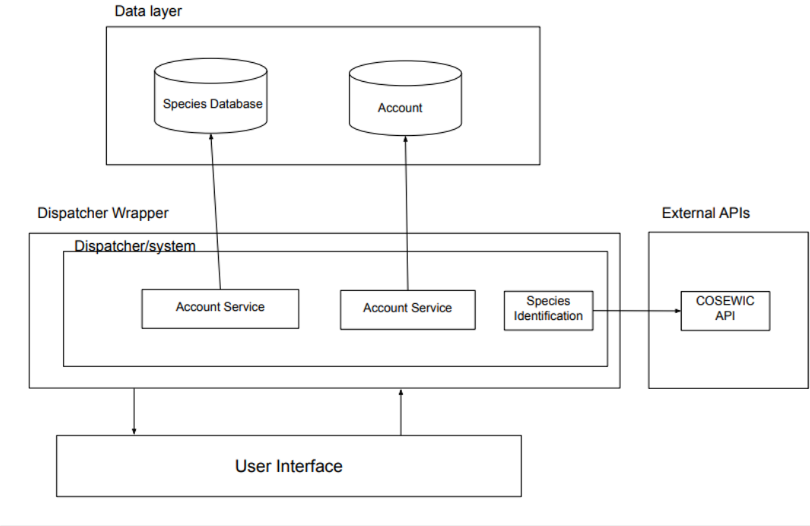
\includegraphics[scale=0.5]{figure1.png}
\end{center}
% End SubSection

\subsection{Product Functions}
\label{sub:product_functions}
% Begin SubSection
The goal of the system is to identify endangered and out of season species for 3 main domains: aerial, aquatic, and land. There will be 3 main methods for identifying specifics and a backend decision tree to determine accuracy and provide a result. The methods will be: description, survey and image. The main modules of this app will be the following: Identifying species (submitting photo, writing a description, filling a questionnaire, getting result), Account Services (creating an account, viewing past inquiries, updating information, logging in), Generate Report (generate report, save results, view accuracy score). 
\begin{center}
    \begin{tabular}{ |p{4cm}|p{10cm}| } 
    \hline
    \textbf{Modules} & \textbf{Functions} \\
    \hline
    Identify Species 
    & \textbf{Write Description}: Allows the user to submit a description of the animal they have seen. \\ 
    & \textbf{Submit Image}: Allows the user to upload an image of animals they see. \\ 
    & \textbf{Fill out Questionnaire}: Allows user to submit an inquiry based on predesigned questions. \\ 
    & \textbf{View Result}: Allows user to see the identified species. \\
    \hline
    Generate Report
    & \textbf{Generate Report}: Allows the user to create a unique report with details of their search and related information. \\ 
    & \textbf{View Score}: Allows the user to see the corresponding accuracy score of generation. \\
    & \textbf{Save Result}: Allows the user to store output. \\
    \hline	
    Account Services 
    & \textbf{Create Account}: Allows the user to create an account. \\ 
    & \textbf{Update Account}: Allows the user to update their account information. \\ 
    & \textbf{Login}: Allows the user to log in or log out of their account. \\ 
    & \textbf{Search History}: Allows the user to view past searches. \\
    \hline
    \end{tabular}
\end{center}


% \begin{center}
% 	\begin{tabular}{ |c|c| } 
% 	\hline
% 	Modules & Functions \\
% 	\hline
% 	Identify Species 
% 	& Write Description: Allows the user to submit a description of the animal they have seen \\ 
%     & Submit Image: Allows the user to upload an image of animals they see \\ 
%     & Fill out Questionnaire: Allows user to submit inquiry based on predesigned questions \\ 
% 	& View Result: Allows user to see the identified species\\
%    \hline
%    Generate Report
%     & Generate report: Allows user to have our system create a unique report entailing details of their search and related infromation\\ 
% 	& View Score: Allows user to see the corresponding accuracy score of generation \\
% 	& Save Result: Allows user to store output \\
% %    Identify Species: Description & Submit Image: Allows the user to upload an image of animals they see \\ 
% %    & View Result: Allows user to see the identified species and corresponding accuracy score \\
% %    & Save Result: Allows user to store output \\
% %   \hline	
% %   \hline
% %   Identify Species: Survey 
% %   & Fill out Questionnaire: Allows user to submit inquiry based on predesigned questions \\ 
% %   & View Result: Allows user to see the identified species and corresponding accuracy score \\
% %   & Save Result: Allows user to store output \\
%  \hline	
%   Account Services & Create Account: Allows the user to create an account\\ 
%   & Update Account: Allows the user to update their account information \\ 
%   & Login: Allows user to login/logout of their account  \\ 
%   & Search History: Allows user to view past searches\\
%  \hline
%    \end{tabular}
% \end{center}
\begin{center}
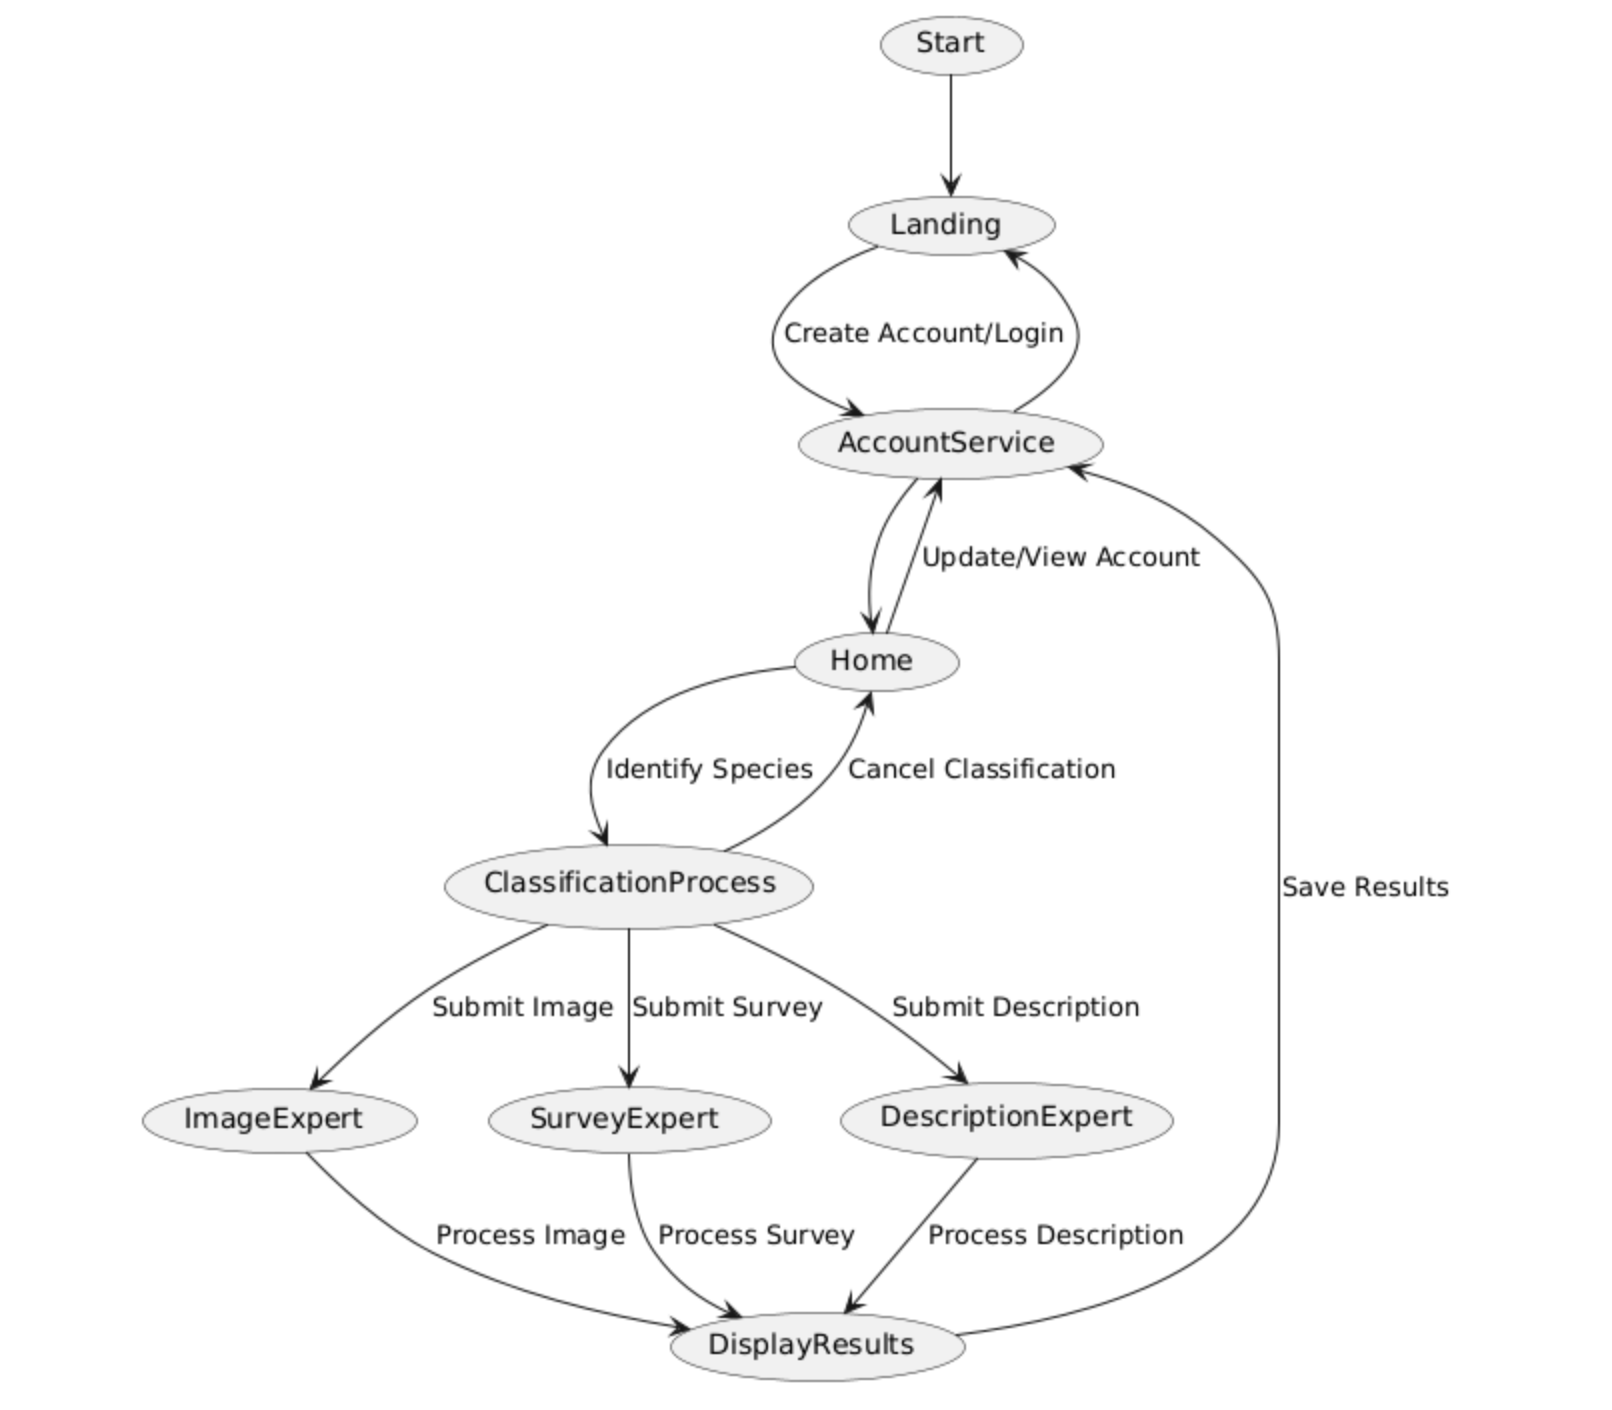
\includegraphics[scale=0.50]{2.2StateDiagram.png}
\end{center}
% End SubSection

\subsection{User Characteristics}
\label{sub:user_characteristics}
\subsubsection{Hunters}
Hunters primarily live in rural areas, sometimes with limited access to educational resources and diverse perspectives. For this reason, they have a majority lower education level 
as those who leave behind their provincial life to gain education in the city may decide to stay there and live behind their rural life of hunting. They have much experience with
 wildlife and its behaviours, many having learned hunting from their parents who in turn learned it from their parents before them. They have, in general,
 a deep respect for wildlife and a vast knowledge of species and their behaviours. However, they may be limited in their knowledge of which species are 
 currently designated to be at risk.
\subsubsection{Nature Enthusiasts}
Nature enthusiasts cover a broad spectrum of people from casual national park-goers to experienced portagers. Their education level varies from those 
who have not graduated high school to those with PhDs and MDs. However, in Canada it tends towards those with undergraduate degrees as that is the most 
common education level. Their experience level varies greatly, however it would tend towards those who camp once or twice a year. Potentially, they have attended 
a seminar run by the national parks and are able to identify a small subset of species. In majority, our user can identify broad spectrums of species (such as moose,
deer, squirrel, bird), but is unable to tell the different nuances between species.
% Begin SubSection
\begin{itemize}
	\item Describe those general characteristics of the intended users of the product including educational level, experience, and technical expertise 
	\item Since there will be many users, you may wish to divide into different user types or personas
%	\item Do not state specific requirements, but rather provide the reasons why certain specific requirements are later specified
\end{itemize}
% End SubSection

\subsection{Constraints}
\label{sub:constraints}
\begin{enumerate}
    \item \textbf{Data Availability:} The accuracy of Gaim depends on an up-to-date and comprehensive database of wildlife species, including their characteristics and at-risk status. Obtaining and maintaining such a database may require collaboration with wildlife organizations and adherence to licensing restrictions. Especially since this is supposed to be Ontario-specific, it will be difficult to obtain such a database.

    \item \textbf{Internet Dependency:} Even though some features can be used locally, features such as cloud-based image processing, AI model updates, and community discussions require an active internet connection. Users in remote locations with limited to no internet connectivity may experience reduced to no functionality.

    \item \textbf{Regulatory and Ethical Constraints:} Since the application deals with wildlife identification, it must comply with Canadian environmental laws and conservation policies. The app must ensure that it does not inadvertently promote illegal activities such as hunting endangered species. Even though the app will provide endangerment status, the list will need to be up-to-date and may require regular checks to stay updated.

    \item \textbf{AI Model Accuracy and Bias:} The AI models used for species identification must be trained with diverse datasets to avoid misclassifications. Ensuring high accuracy while maintaining real-time performance is a key challenge, as incorrect identifications may mislead users. This can be especially critical with endangered species and protected species.

    \item \textbf{Scalability:} As Gaim gains more users, the system must be capable of handling increased data processing demands and community interactions. Future versions may require cloud infrastructure scaling, which could introduce additional costs. 
\end{enumerate}

\subsection{Assumptions and Dependencies}
\label{sub:assumptions_and_dependencies}
% Begin SubSection
\begin{itemize}
	\item Audio recordings are clear and free of excessive background noise.
	\item Images and videos are of sufficient resolution, clarity, and lighting for accurate identification.
    \item The app will only be used in Canada (no need to consider species from other regions).
    \item We have access to cloud or local computational resources to handle image and sound processing.
    \item Assume APIs are secure and functional
    \item Assume user has internet connection
    
\end{itemize}

% End SubSection

\subsection{Apportioning of Requirements}
\label{sub:apportioning_of_requirements}
% Begin SubSection
\begin{itemize}
	\item The first version of the app will not take into consideration animals whose appearances change by season.
    \item The first version of the app will be developed in English.
    \item Verify with wildlife experts to check accuracy of our results.
    \item Expand database to take into account species from other regions as the app grows.
\end{itemize}
% End SubSection
% End Section
\section{Use Case Diagram}
\label{sec:use_case_diagram}
\begin{center}
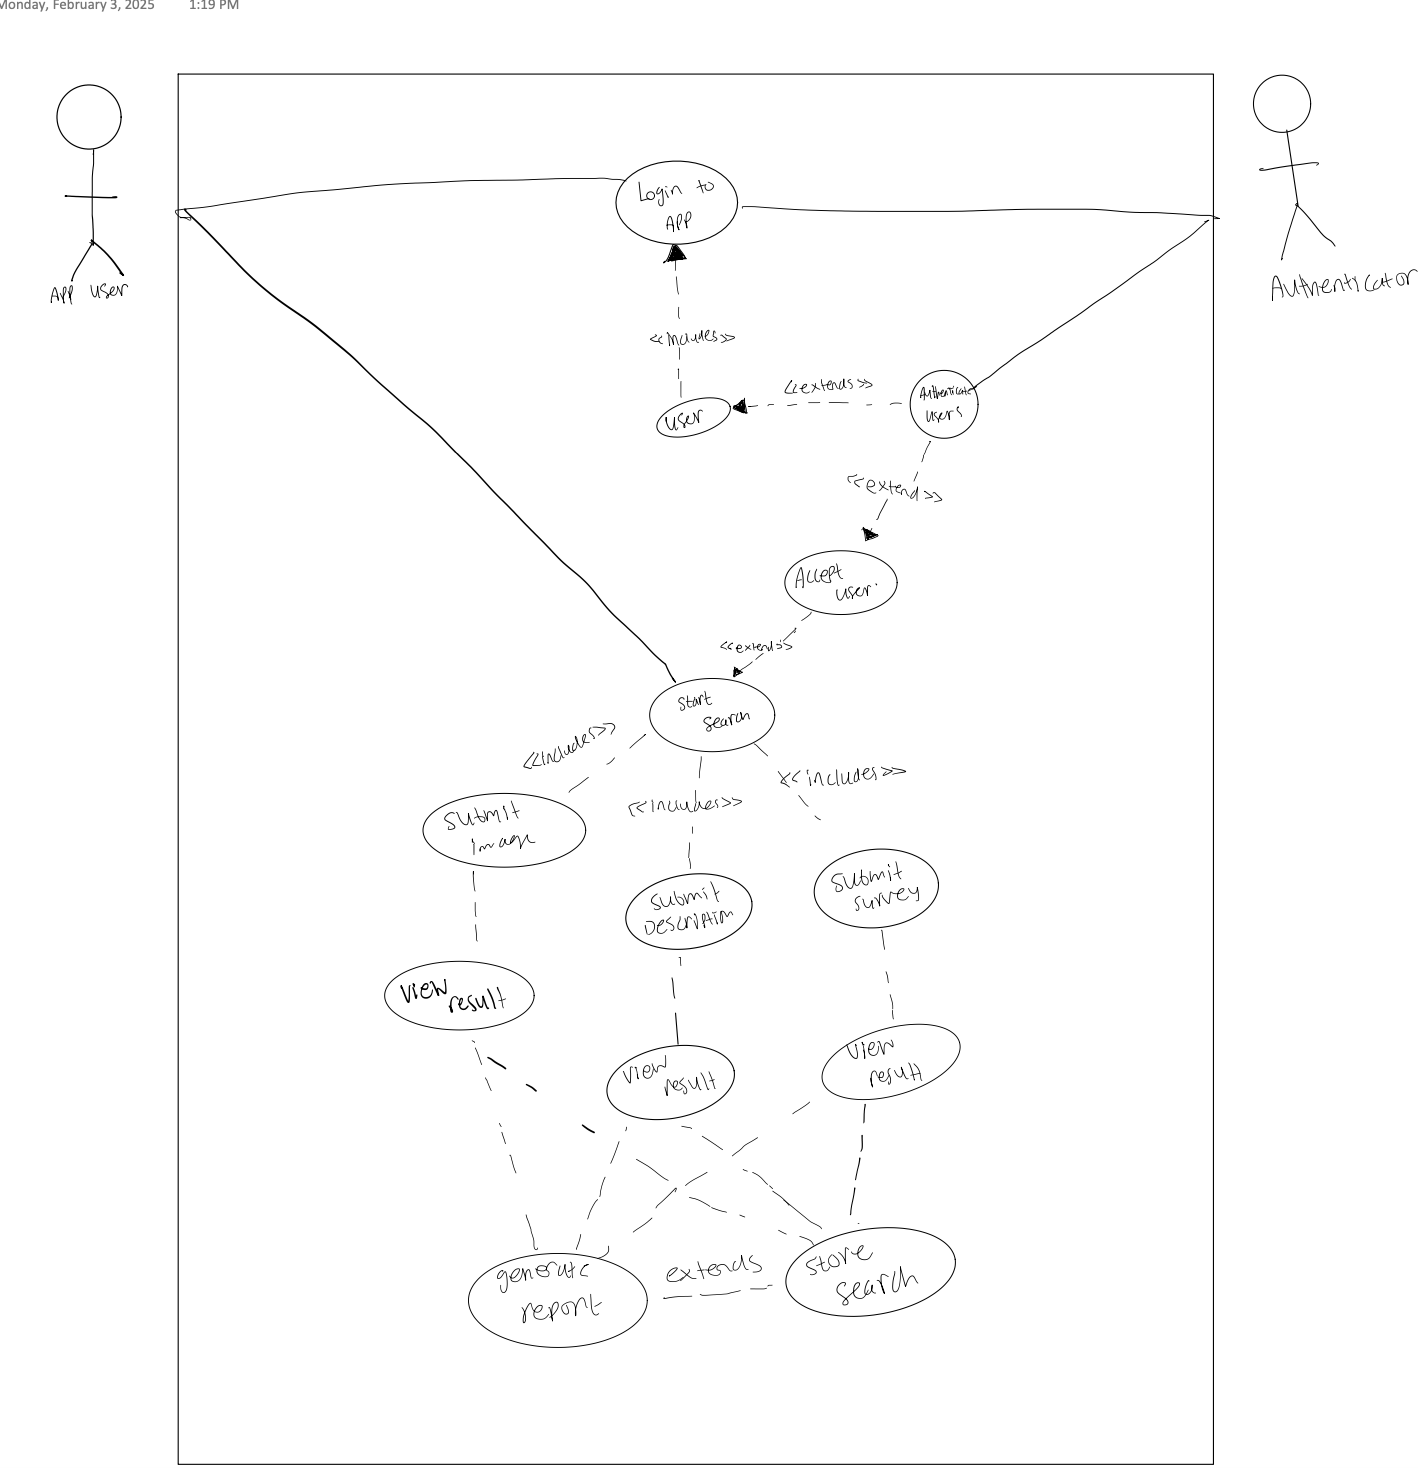
\includegraphics[scale=0.75]{3Diagram.png}
\end{center}
% Begin Section
% \begin{itemize}
% 	\item Provide the use case diagram for the system being developed.
% 	\item You do not need to provide the textual description of any of the use cases here (these will be specified under "Highlights of Functional Requirements").
% %	\item Provide \emph{one} use case diagram for the most important Business Event.
% %	\item The text of all use cases will be specified under "Highlights of Functional Requirements"
% \end{itemize}
%In this section, select the most important Business Event that your system responds to and give its use case diagram.  Only one use case diagram is needed.  Give a brief textual description of the use case without repeating what is in the scenarios of the corresponding Business Event.

%
%
%
%This section should provide a use case diagram for your application. 
%\begin{enumerate}[a)]
%	\item Each use case appearing in the diagram should be accompanied by a text description. 
%\end{enumerate}
%% End Section

\section{Highlights of Functional Requirements}
\label{sec:functional_requirements}
% Begin Section
% \begin{itemize}
% 	\item Specify all use cases (or other scenarios triggered by other events), organized by Business Event. 
% 	\item For each Business Event, show the scenario from every Viewpoint. You should have the same set of Viewpoints across all Business Events. If a Viewpoint doesn't participate, write N/A so we know you considered it still. You can choose how to present this - keep in mind it should be easy to follow. 
% 	\item At the end, combine them all into a Global Scenario.
% 	%\item Specify the "use cases" (or other triggering events) organized by Business Event. (The Global Scenario is what you might think of as a use case). Be sure to consider Business Events that aren't just triggered by users with goals (e.g. something happens in the environment that your system needs to respond to)
% 	\item Your focus should be on what the system needs to do, not how to do it. Specify it in enough detail that it clearly specifies what needs to be accomplished, but not so detailed that you start programming or making design decisions.
% 	\item Keep the length of each use case (Global Scenario) manageable. If it's getting too long, split into sub-cases.
% 	\item You are \emph{not} specifying a complete and consistent set of functional requirements here. (i.e. you are providing them in the form of use cases/global scenarios, not a refined list). For the purpose of this project, you do not need to reduce them to a list; the global scenarios format is all you need.
% 	\item Red text below is just to highlight where you need to insert a scenario - don't actually write it all in red.
% \end{itemize}
\noindent {\bf Main Business Events:} List out all the main business events you are presenting. If you sub-divided into smaller ones, you don't need to include the smaller ones in this list.\\

\noindent {\bf Viewpoints:} List out all the viewpoints you will be considering.\\

\noindent {\bf Interpretation:} Specify any liberties you took in interpreting business events, if necessary.\\

\begin{enumerate}[{\bf BE1.}]
	\item Business Event Name \#1
		\begin{enumerate}[{\bf VP1.}]
			\item Viewpoint Name \#1 \\
				\textcolor{red}{Insert Scenario Here}
			\item Viewpoint Name \#2 \\
				\textcolor{red}{Insert Scenario Here}
		\end{enumerate}
		{\bf Global Scenario:}\\
		\textcolor{red}{Insert Scenario Here}
	\item Business Event Name \#2
	\begin{enumerate}[{\bf VP1.}]
		\item Viewpoint Name \#1 \\
		\textcolor{red}{Insert Scenario Here}
		\item Viewpoint Name \#2 \\
		\textcolor{red}{Insert Scenario Here}
	\end{enumerate}
	{\bf Global Scenario:}\\
	\textcolor{red}{Insert Scenario Here}

    \item Submitting a photo \#3

    \textbf{Precondition:} The user has an account and is logged into the system. The user has captured or selected an image of an animal to be analyzed.

	\begin{enumerate}[{\bf VP1.}]
		\item User \#1 \\
		
            \textbf{Main Success Scenario:}
            \begin{enumerate}
    \item[1] User opens the application on their mobile device.
    \item[2] System requires the user to log in and displays the login fields.
    \item[3] User enters their account credentials.
    \item[4] System authenticates the user.
    \item[5] User selects the "Identify Species" option.
    \item[6] System prompts the user to upload an image from their gallery or take a new photo.
    \item[7] User selects or captures an image.
    \item[8] System uploads the image and begins processing using the Image Recognition Expert.
    \item[9] Image Recognition Expert generates a prediction of the species along with an accuracy score.
    \item[10] The system forwards the prediction and accuracy score to the central forum.
    \item[11] The forum waits for inputs from the other experts before finalizing a decision.
    \item[12] System displays a "Processing Submission" status to the user.
    \item[13] Once all expert opinions are collected, the forum finalizes the species identification.
    \item[14] System displays the identified species, confidence level, and additional relevant details to the user.

    \end{enumerate}

    \textbf{Secondary Scenarios:}
    \begin{itemize}
    \item 4i. System fails to authenticate the user.
    \begin{enumerate}
        \item[4i.1] System fails to authenticate the user.
        \item[4i.2] System prompts the user to reset their password or contact support.
    \end{enumerate}
    
    \item 8i. User submits an invalid or blurry image.
    \begin{enumerate}
        \item[8i.1] System detects that the image is too blurry or invalid.
        \item[8i.2] System prompts the user to submit a clearer image.
    \end{enumerate}

    \item 9i. Image Recognition Expert fails to generate a prediction.
    \begin{enumerate}
        \item[9i.1] System fails to generate a prediction due to insufficient data.
        \item[9i.2] System notifies the user and suggests using another identification method (e.g., text description or survey).
    \end{enumerate}

    \item 13i. Other experts fail to provide input to the forum.
    \begin{enumerate}
        \item[13i.1] The forum detects missing inputs from other experts.
        \item[13i.2] The system returns a partial result based on available data and notifies the user.
    \end{enumerate}
\end{itemize}
    

		\item Ads Team \#2 \\
\begin{enumerate}
    \item [12i.1] System logs the user's engagement with the image submission feature.
    \item [12i.2] If applicable, the system selects wildlife-related advertisements based on the submission context.
    \item [12i.3] The system ensures that advertisements do not disrupt the user experience.
\end{enumerate}

            \item Marketing Team \#3 \\
\begin{enumerate}
    \item [12i.4] System tracks user engagement data related to photo submissions.
    \item [12i.5] System collects data for analytics to improve user experience and optimize future marketing strategies.
\end{enumerate}


            \item Accounting Team \#4 \\
        \newline NA


        \item Environment Canada \#5 \\
\begin{enumerate}
    \item[8ii.1] System  flags any identified endangered or protected species.
    \item[8ii.2]    System flagged submissions for regulatory tracking.
    \item[8ii.3] If applicable, the system notifies the appropriate authorities about the flagged species.
\end{enumerate}



\item National Parks/Hunting Organization (Ontario Federation of Anglers and Hunters) \#6 \\
\begin{enumerate}
    \item [8iii.1] System logs identified species data for conservation efforts and hunting regulations.
    \item[8iii.2] If the species is considered *unhuntable* due to conservation laws, the system notifies the user.
    \item[8iii.3] System provides relevant legal hunting information based on the identified species.
\end{enumerate}
    \textbf{Global Scenario:}

    \noindent \textbf{Pre-condition:}  
User is logged in and submits a photo for species identification.

\noindent \textbf{Main Success Scenario:}
\begin{enumerate}
    \item User uploads or captures an image.
    \item System processes the image using AI models.
    \item System submits results to the forum.
    \item Forum consolidates data from all identification experts.
    \item Final species prediction is displayed to the user.
    \item User can choose to submit the identification result to the community.
\end{enumerate}

\noindent \textbf{Secondary Scenarios:}
\begin{itemize}
    \item If the system fails to authenticate the user, it prompts for login recovery.
    \item If the image is invalid, the user is asked to submit another one.
    \item If the Image Recognition Expert fails, the user is advised to use another input method.
    \item If some experts fail to respond, the forum provides an answer based on available data.
\end{itemize}
\end{enumerate}

\item Submitting a survey \#4

    \textbf{Precondition:} The user has an account and is logged into the system. The user has chosen to identify an animal using the survey-based method.

	\begin{enumerate}[{\bf VP1.}]
		\item User \#1 \\
		
            \textbf{Main Success Scenario:}
            \begin{enumerate}
                \item[1] User opens the application on their mobile device.
                \item[2] System requires the user to log in and displays the login fields.
                \item[3] User enters their account credentials.
                \item[4] System authenticates the user.
                \item[5] User selects the "Identify Species" option.
                \item[6] System prompts the user to choose a method: Image-based or Survey-based identification.
                \item[7] User selects the Survey-based identification.
                \item[8] System initiates the Decision-Tree Expert and starts the questionnaire.
                \item[9] System presents the first question, prompting the user with a yes/no or multiple-choice format.
                \item[10] User responds to each question, and based on the responses, the Decision-Tree Expert dynamically adjusts the next question.
                \item[11] The Decision-Tree Expert continues until it determines a probable species or exhausts all questions.
                \item[12] System generates a prediction of the species along with an accuracy score.
                \item[13] The system forwards the prediction and accuracy score to the central forum.
                \item[14] The forum waits for inputs from the other experts before finalizing a decision.
                \item[15] System displays a "Processing Submission" status to the user.
                \item[16] Once all expert opinions are collected, the forum finalizes the species identification.
                \item[17] System displays the identified species, confidence level, and additional relevant details to the user.
            \end{enumerate}

    \textbf{Secondary Scenarios:}
    \begin{itemize}
        \item 4i. System fails to authenticate the user.
        \begin{enumerate}
            \item[4i.1] System fails to authenticate the user.
            \item[4i.2] System prompts the user to reset their password or contact support.
        \end{enumerate}
        
        \item 8i. User provides inconsistent or conflicting answers in the survey.
        \begin{enumerate}
            \item[8i.1] System detects logical inconsistencies in the user's responses.
            \item[8i.2] System prompts the user to review their answers or restart the survey.
        \end{enumerate}

        \item 12i. Decision-Tree Expert fails to generate a prediction.
        \begin{enumerate}
            \item[12i.1] System fails to determine a probable species due to insufficient matching data.
            \item[12i.2] System notifies the user and suggests using another identification method (e.g., image-based or freeform text description).
        \end{enumerate}

        \item 13i. Other experts fail to provide input to the forum.
        \begin{enumerate}
            \item[13i.1] The forum detects missing inputs from other experts.
            \item[13i.2] The system returns a partial result based on available data and notifies the user.
        \end{enumerate}
    \end{itemize}
    

		\item Ads Team \#2 \\
\begin{enumerate}
    \item [12i.3] System logs the user's engagement with the survey submission feature.
    \item [12i.4] If applicable, the system selects wildlife-related advertisements based on the submission context.
    \item [12i.5] The system ensures that advertisements do not disrupt the user experience.
\end{enumerate}

        \item Marketing Team \#3 \\
\begin{enumerate}
    \item [12i.6] System tracks user engagement data related to survey submissions.
    \item [12i.7] System collects data for analytics to improve user experience and optimize future marketing strategies.
\end{enumerate}

        \item Accounting Team \#4 \\
        \newline NA

        \item Environment Canada \#5 \\
\begin{enumerate}
    \item[8ii.1] System flags any identified endangered or protected species.
    \item[8ii.2] System logs flagged submissions for regulatory tracking.
    \item[8ii.3] If applicable, the system notifies the appropriate authorities about the flagged species.
\end{enumerate}

        \item National Parks/Hunting Organization (Ontario Federation of Anglers and Hunters) \#6 \\
\begin{enumerate}
    \item [8iii.1] System logs identified species data for conservation efforts and hunting regulations.
    \item[8iii.2] If the species is considered *unhuntable* due to conservation laws, the system notifies the user.
    \item[8iii.3] System provides relevant legal hunting information based on the identified species.
\end{enumerate}
        
\end{enumerate}

\textbf{Global Scenario:}

\textbf{Precondition:} The user has an account and is logged into the system.

\textbf{Main Success Scenario:}
\begin{enumerate}
    \item User selects survey-based species identification.
    \item System presents a series of questions dynamically based on the Decision-Tree Expert.
    \item User completes the survey.
    \item System generates a species prediction and accuracy score.
    \item System submits results to the forum.
    \item Forum consolidates data from all identification experts.
    \item Final species prediction is displayed to the user.
    \item User can choose to submit the identification result to the community.
\end{enumerate}

\textbf{Secondary Scenarios:}
\begin{itemize}
    \item If the system fails to authenticate the user, it prompts for login recovery.
    \item If the survey responses are inconsistent, the user is asked to review or restart the survey.
    \item If the Decision-Tree Expert fails to generate a prediction, the user is advised to use another input method.
    \item If some experts fail to respond, the forum provides an answer based on available data.
\end{itemize}
\item Editing Account \#5
 
\textbf{Precondition:} Has an account and is trying to change account details.
 
\begin{enumerate}[{\bf VP1.}]
\item User \#1 \
 
    \textbf{Main Success Scenario:}
    \begin{enumerate}
        \item[1] User navigates to the "Edit Account" page.
        \item[2] User modifies account details (e.g., name, email, password).
        \item[3] System validates the input.
        \item[4] If validation succeeds, the system updates the database.
        \item[5] User receives a confirmation message.
        \item[6] If validation fails, the system displays an error message and prompts the user for corrections.
    \end{enumerate}
 
\textbf{Secondary Scenarios:}
\begin{itemize}
\item 4i. User provides invalid input.
\begin{enumerate}
\item[4i.1] System detects invalid input.
\item[4i.2] System prompts the user to correct the information and retry.
\end{enumerate}
\end{itemize}
 
\item Ads Team \#2 \
\begin{enumerate}
\item N/A (The Ads Team has no role in the editing account process.)
\end{enumerate}
 
\item Marketing Team \#3 \
\begin{enumerate}
\item N/A (The Marketing Team does not directly interact with the editing account system.)
\end{enumerate}
 
\item Accounting Team \#4 \
\begin{enumerate}
\item (a) User updates billing information.
\item (b) The system validates the changes.
\item (c) The accounting team’s module is updated to reflect new details.
\item (d) Confirmation is sent to the user.
\end{enumerate}
 
\item Environment Canada \#5 \
\begin{enumerate}
\item N/A (Environment Canada has no involvement in the editing account process.)
\end{enumerate}
 
\item National Parks/Hunting Organization (Ontario Federation of Anglers and Hunters) \#6 \
\begin{enumerate}
\item N/A (This organization has no involvement in the editing account process.)
\end{enumerate}
\end{enumerate}
 
\textbf{Global Scenario:}
 
\textbf{Precondition:}
 
\textbf{Main Success Scenario:}
\begin{enumerate}
\item User accesses the "Edit Account" page.
\item User modifies account details.
\item System validates the input.
\item If validation succeeds, the system updates the database.
\item User receives a confirmation message.
\item If validation fails, the system displays an error message and prompts the user for corrections.
\end{enumerate}
 
\textbf{Secondary Scenarios:}
\begin{itemize}
\item If the user provides invalid input, the system prompts for corrections.
\item If billing information is updated, the accounting module is notified.
\end{itemize}
 
 
\item Login \#6
 
\textbf{Precondition:} Has an account and is trying to log in.
 
\begin{enumerate}[{\bf VP1.}]
\item User \#1 \
 
    \textbf{Main Success Scenario:}
    \begin{enumerate}
        \item[1] User navigates to the login page.
        \item[2] User inputs their credentials (email/username and password).
        \item[3] System validates the credentials.
        \item[4] If credentials match, access is granted, and the user is redirected to their dashboard.
        \item[5] If credentials do not match, the system displays an error message and allows the user to retry or reset the password.
    \end{enumerate}
 
\textbf{Secondary Scenarios:}
\begin{itemize}
\item 4i. User has overdue payments.
\begin{enumerate}
\item[4i.1] System flags the account and restricts access until the payment issue is resolved.
\item[4i.2] User is notified of the restriction and given options to settle the issue.
\end{enumerate}
\end{itemize}
 
\item Ads Team \#2 \
\begin{enumerate}
\item N/A (The Ads Team has no role in the login process.)
\end{enumerate}
 
\item Marketing Team \#3 \
\begin{enumerate}
\item N/A (The Marketing Team does not directly interact with the login system.)
\end{enumerate}
 
\item Accounting Team \#4 \
\begin{enumerate}
\item (a) User with overdue payments attempts to log in.
\item (b) The system flags the account and restricts access until the payment issue is resolved.
\item (c) User is notified of the restriction and given options to settle the issue.
\end{enumerate}
 
\item Environment Canada \#5 
\begin{enumerate}
\item N/A (Environment Canada has no involvement in the login process.)
\end{enumerate}
 
\item National Parks/Hunting Organization (Ontario Federation of Anglers and Hunters) \#6 \
\begin{enumerate}
\item N/A (This organization has no involvement in the login process.)
\end{enumerate}
\end{enumerate}
 
\textbf{Global Scenario:}
 
\textbf{Precondition:}
 
\textbf{Main Success Scenario:}
\begin{enumerate}
\item User navigates to the login page.
\item User inputs their credentials.
\item System validates the credentials.
\item If credentials match, access is granted, and the user is redirected to their dashboard.
\item If credentials do not match, the system displays an error message and allows the user to retry or reset the password.
\end{enumerate}
 
\textbf{Secondary Scenarios:}
\begin{itemize}
\item If the user has overdue payments, the system flags the account and restricts access until payment is settled.
\item User is notified of the restriction and provided with payment options.
\end{itemize}

\item Viewing a Report \#7

    \textbf{Precondition:} The user has already taken a picture of an animal and the forum has generated a report.

    \begin{enumerate}[{\bf VP1.}]
        \item User \#1 \\

            \textbf{Main Success Scenario:}
            \begin{enumerate}
                \item[1] The user opens the app and logs in.
                \item[2] The system authenticates the user and displays the dashboard.
                \item[3] The user selects "View Report" from the options.
                \item[4] The system displays a list of available reports.
                \item[5] The user selects a specific report from the list.
                \item[6] The system retrieves the report details and displays them to the user, including the animal's name, species, habitat, diet, and conservation status.
            \end{enumerate}

            \textbf{Secondary Scenario:}
            \begin{enumerate}
                \item[4i] System fails to retrieve the list of reports.
                \begin{enumerate}
                    \item[4i.1] The system displays an error message.
                    \item[4i.2] The user is prompted to try again or contact customer support.
                \end{enumerate}
                \item[5i] System fails to display the report content.
                \begin{enumerate}
                    \item[5i.1] System displays a “Report Unavailable" message.
                    \item[5i.2] The user is prompted to reload the report or connect with customer support.
                \end{enumerate}
            \end{enumerate}
    \end{enumerate}

    \begin{enumerate}[{\bf VP2.}]
        \item Ads Team \\ 
        N/A
    \end{enumerate}

    \begin{enumerate}[{\bf VP3.}]
        \item Marketing Team \\
        N/A
    \end{enumerate}

    \begin{enumerate}[{\bf VP4.}]
        \item Accounting Team \\
        N/A
    \end{enumerate}

    \begin{enumerate}[{\bf VP5.}]
        \item Environment Canada \\
        N/A
    \end{enumerate}

    \begin{enumerate}[{\bf VP6.}]
        \item National Parks/Hunting Organization \\
        N/A
    \end{enumerate}

    \textbf{Global Scenario:} \\
    \textbf{Precondition:} The user has an account and is logged into the system. A report has already been generated for the image taken by the user. \\

    \textbf{Main Success Scenario:}
    \begin{enumerate}
        \item[(a)] User selects "View Report" from the dashboard.
        \item[(b)] The system retrieves and displays the report information, including the animal's details such as species, habitat, and diet.
        \item[(c)] User reviews the report.
        \item[(d)] User may choose to share the report with the community.
    \end{enumerate}

    \textbf{Secondary Scenarios:}
    \begin{itemize}
        \item If the system fails to authenticate the user, it prompts for login recovery.
        \item If the report fails to load, the user is prompted to refresh or contact customer support.
        \item If the report data is incomplete, the system displays a warning and suggests a re-scan.
    \end{itemize}

\item Saving a Report \#8

    \textbf{Precondition:} The user is viewing a generated report and wants to save it for offline access or future reference.

    \begin{enumerate}[{\bf VP1.}]
        \item User \#1 \\

            \textbf{Main Success Scenario:}
            \begin{enumerate}
                \item[1] The user opens the app and logs in.
                \item[2] The system authenticates the user.
                \item[3] The user views the generated report.
                \item[4] The user selects the Save Report option
                \item[5] The system prompts the user to choose a format (e.g., PDF, Image) and confirm the save.
                \item[6] The user confirms the action.
                \item[7] The system saves the report to the user’s device and provides a success message.
            \end{enumerate}

            \textbf{Secondary Scenario:}
            \begin{enumerate}
                \item[3i] User selects an unsupported format.
                \begin{enumerate}
                    \item[3i.1] System displays an "Unsupported Format" message and prompts the user to select a valid format.
                \end{enumerate}
                \item[4i] System fails to save the report.
                \begin{enumerate}
                    \item[4i.1] System displays a "Save Failed" error message.
                    \item[4i.2] User is prompted to try saving again or contact customer support.
                \end{enumerate}
            \end{enumerate}
    \end{enumerate}

    \begin{enumerate}[{\bf VP2.}]
        \item Ads Team \\ 
        N/A
    \end{enumerate}

    \begin{enumerate}[{\bf VP3.}]
        \item Marketing Team \\
        N/A
    \end{enumerate}

    \begin{enumerate}[{\bf VP4.}]
        \item Accounting Team \\
        N/A
    \end{enumerate}

    \begin{enumerate}[{\bf VP5.}]
        \item Environment Canada \\
        N/A
    \end{enumerate}

    \begin{enumerate}[{\bf VP6.}]
        \item National Parks/Hunting Organization \\
        N/A
    \end{enumerate}


\textbf{Global Scenario:} \\
    \textbf{Precondition:} The user has an account and is logged into the system, and a report has already been generated. \\
    \textbf{Main Success Scenario:}
            \begin{enumerate}
                \item[1] The user opens the app and logs in.
                \item[2] The system authenticates the user.
                \item[3] The user views the generated report.
                \item[4] The user selects the Save Report option
                \item[5] The system prompts the user to choose a format (e.g., PDF, Image) and confirm the save.
                \item[6] The user confirms the action.
                \item[7] The system saves the report to the user’s device and provides a success message.
            \end{enumerate}

            \textbf{Secondary Scenario:}
            \begin{enumerate}
                \item[3i] User selects an unsupported format.
                \begin{enumerate}
                    \item[3i.1] System displays an "Unsupported Format" message and prompts the user to select a valid format.
                \end{enumerate}
                \item[4i] System fails to save the report.
                \begin{enumerate}
                    \item[4i.1] System displays a "Save Failed" error message.
                    \item[4i.2] User is prompted to try saving again or contact customer support.
                \end{enumerate}
            \end{enumerate}
    

\end{enumerate}

%	Below, we organize by Business Event.
%	\begin{enumerate}[{BE}1.]
%		\item Business Event name
%		\begin{enumerate}[{VP1}.1]
%			\item Viewpoint name \newline
%			\noindent\fbox{%
%				\parbox{0.5\textwidth}{%
%					\begin{itemize}
%						\item {\bf $S_{1}$:} Initial response of the system to the Business Event
%						\item {\bf $E_{1}$:}  Reaction of the environment to $S_{1}$
%						\item {\bf $S_{2}$:}  Response of the system to $E_{1}$
%						\item {\bf $E_{2}$:}  Reaction of the environment to $S_{2}$
%						\item[] $\cdots$
%						\item {\bf $S_{n}$:}  Response of the system to $E_{(n-1)}$
%						\item {\bf $E_{n}$:}  Reaction of the environment to $E_{(n-1)}$
%						\item {\bf $S_{(n+1)}$:} Final response of the system concluding its function regarding the Business Event
%					\end{itemize}
%				}%
%			}
%			\item Viewpoint name\newline
%			\noindent\fbox{%
%				\parbox{0.5\textwidth}{%
%					\begin{itemize}
%						\item {\bf $S_{1}$:} Initial response of the system to the Business Event
%						\item {\bf $E_{1}$:}  Reaction of the environment to $S_{1}$
%						\item {\bf $S_{2}$:}  Response of the system to $E_{1}$
%						\item {\bf $E_{2}$:}  Reaction of the environment to $S_{2}$
%						\item[] $\cdots$
%						\item {\bf $S_{k}$:}  Response of the system to $E_{(k-1)}$
%						\item {\bf $E_{k}$:}  Reaction of the environment to $E_{(k-1)}$
%						\item {\bf $S_{(k+1)}$:} Final response of the system concluding its function regarding the Business Event
%					\end{itemize}
%				}%
%			}
%			\item \dots
%			\item \dots
%			\item \dots
%			\item[\dots]
%		\end{enumerate}	
%		\item[] {\bf Global Scenario of {\it Business Event Name}:} It is the scenario corresponding to the integration of all the above scenarios from the different Viewpoints of the Business Event BE1.\newline
%		\noindent\fbox{%
%			\parbox{0.5\textwidth}{%
%				\begin{itemize}
%					\item {\bf $S_{1}$:} Initial response of the system to the Business Event
%					\item {\bf $E_{1}$:}  Reaction of the environment to $S_{1}$
%					\item {\bf $S_{2}$:}  Response of the system to $E_{1}$
%					\item {\bf $E_{2}$:}  Reaction of the environment to $S_{2}$
%					\item[] $\cdots$
%					\item {\bf $S_{m}$:}  Response of the system to $E_{(m-1)}$
%					\item {\bf $E_{m}$:}  Reaction of the environment to $E_{(m-1)}$
%					\item {\bf $S_{(m+1)}$:} Final response of the system concluding its function regarding the Business Event
%				\end{itemize}
%			}%
%		}	
%		%\end{enumerate}
%		\item Business Event name
%		\begin{enumerate}[{VP1}.1]
%			\item Viewpoint name \newline
%			\noindent\fbox{%
%				\parbox{0.5\textwidth}{%
%					\begin{itemize}
%						\item {\bf $S_{1}$:} Initial response of the system to the Business Event
%						\item {\bf $E_{1}$:}  Reaction of the environment to $S_{1}$
%						\item {\bf $S_{2}$:}  Response of the system to $E_{1}$
%						\item {\bf $E_{2}$:}  Reaction of the environment to $S_{2}$
%						\item[] $\cdots$
%						\item {\bf $S_{n'}$:}  Response of the system to $E_{(n'-1)}$
%						\item {\bf $E_{n'}$:}  Reaction of the environment to $E_{(n'-1)}$
%						\item {\bf $S_{(n'+1)}$:} Final response of the system concluding its function regarding the Business Event
%					\end{itemize}
%				}%
%			}
%			\item Viewpoint name\newline
%			\noindent\fbox{%
%				\parbox{0.5\textwidth}{%
%					\begin{itemize}
%						\item {\bf $S_{1}$:} Initial response of the system to the Business Event
%						\item {\bf $E_{1}$:}  Reaction of the environment to $S_{1}$
%						\item {\bf $S_{2}$:}  Response of the system to $E_{1}$
%						\item {\bf $E_{2}$:}  Reaction of the environment to $S_{2}$
%						\item[] $\cdots$
%						\item {\bf $S_{k'}$:}  Response of the system to $E_{(k'-1)}$
%						\item {\bf $E_{k'}$:}  Reaction of the environment to $E_{(k'-1)}$
%						\item {\bf $S_{(k'+1)}$:} Final response of the system concluding its function regarding the Business Event
%					\end{itemize}
%				}%
%			}
%			\item \dots
%			\item \dots
%			\item \dots
%			\item[\dots]
%		\end{enumerate}	
%		\item[] {\bf Global Scenario of {\it Business Event Name}:} It is the scenario corresponding to the integration of all the above scenarios from the different Viewpoints of the Business Event BE2.\newline
%		\noindent\fbox{%
%			\parbox{0.5\textwidth}{%
%				\begin{itemize}
%					\item {\bf $S_{1}$:} Initial response of the system to the Business Event
%					\item {\bf $E_{1}$:}  Reaction of the environment to $S_{1}$
%					\item {\bf $S_{2}$:}  Response of the system to $E_{1}$
%					\item {\bf $E_{2}$:}  Reaction of the environment to $S_{2}$
%					\item[] $\cdots$
%					\item {\bf $S_{m'}$:}  Response of the system to $E_{(m'-1)}$
%					\item {\bf $E_{m'}$:}  Reaction of the environment to $E_{(m'-1)}$
%					\item {\bf $S_{(m'+1)}$:} Final response of the system concluding its function regarding the Business Event
%				\end{itemize}
%			}%
%		}		
%	\end{enumerate}

%End Section

\section{Non-Functional Requirements}
\label{sec:non-functional_requirements}


\begin{itemize}
	\item For each non-functional requirement, provide a justification/rationale for it.\\
	{\bf Example:} \\
	SC1. \emph{The device should not explode in a customer’s pocket.}\\
	{\bf Rationale:} Other companies have had issues with the batteries they used in their phones randomly exploding [insert citation]. This causes a safety issue, as the phone is often carried in a person's hand or pocket.	
	\item If you need to make a guess because you couldn't really talk to stakeholders, you can say "We imagined stakeholders would want...because..."
	\item Each requirement should have a unique label/number for it.
	\item In the list below, if a particular section doesn't apply, just write N/A so we know you considered it.
\end{itemize}

% Begin Section
\subsection{Look and Feel Requirements}
\label{sub:look_and_feel_requirements}
% Begin SubSection

\subsubsection{Appearance Requirements}
\label{ssub:appearance_requirements}
% Begin SubSubSection
\begin{enumerate}[{LF-A}1. ]
	\item 
\end{enumerate}
% End SubSubSection

\subsubsection{Style Requirements}
\label{ssub:style_requirements}
% Begin SubSubSection
\begin{enumerate}[{LF-S}1. ]
	\item 
\end{enumerate}
% End SubSubSection

% End SubSection

\subsection{Usability and Humanity Requirements}
\label{sub:usability_and_humanity_requirements}
% Begin SubSection

\subsubsection{Ease of Use Requirements}
\label{ssub:ease_of_use_requirements}
% Begin SubSubSection
\begin{enumerate}[{UH-EOU}1. ]
	\item 
\end{enumerate}
% End SubSubSection

\subsubsection{Personalization and Internationalization Requirements}
\label{ssub:personalization_and_internationalization_requirements}
% Begin SubSubSection
\begin{enumerate}[{UH-PI}1. ]
	\item 
\end{enumerate}
% End SubSubSection

\subsubsection{Learning Requirements}
\label{ssub:learning_requirements}
% Begin SubSubSection
\begin{enumerate}[{UH-L}1. ]
	\item 
\end{enumerate}
% End SubSubSection

\subsubsection{Understandability and Politeness Requirements}
\label{ssub:understandability_and_politeness_requirements}
% Begin SubSubSection
\begin{enumerate}[{UH-UP}1. ]
	\item 
\end{enumerate}
% End SubSubSection

\subsubsection{Accessibility Requirements}
\label{ssub:accessibility_requirements}
% Begin SubSubSection
\begin{enumerate}[{UH-A}1. ]
	\item 
\end{enumerate}
% End SubSubSection

% End SubSection
\subsection{Performance Requirements}
\label{sub:performance_requirements}
% Begin SubSection

\subsubsection{Speed and Latency Requirements}
\label{ssub:speed_and_latency_requirements}
% Begin SubSubSection
\begin{enumerate}[{PR-SL}1. ]
	\item The response time of all external APIs (expert calls, database updates, report generation, etc.) should be within 0.5 seconds.
	\newline  \textbf{Rationale:} The average API response time is between 100ms to 500ms [1] and this is known as the typical expectation of performance. A response time in this range is expected by industry standards and is required for a competitive user experience. We would ideally want limited delays, to promote efficiency and satisfaction, and this API response time will ensure that. 
	\item App start-up time should be around 2 seconds.
	\newline  \textbf{Rationale:} The average start-up time in the industry is around 1.5 to 4 seconds [2]. This is the time frame that most systems and users typically wait for. Creating an application that does not fit these requirements will cause us to lose user interest. 
	\item Account updates should be within 3 seconds.
	\newline \textbf{Rationale:} When a user updates their account to save a report, update personal data or look for items previously stored our system should efficiently fetch this information from our database. This is the most time it should take for old information to be requested, searched and displayed on the user screen [3].
\end{enumerate}
% End SubSubSection

\subsubsection{Safety-Critical Requirements}
\label{ssub:safety_critical_requirements}
% Begin SubSubSection
\begin{enumerate}[{PR-SC}1. ]
	\item The app should provide safe suggestions for user reports.
	\newline \textbf{Rationale:} Since our app targets natural areas and focuses on the hunting community recommendations we give during our report generation must be as safe as possible. Focus there is always room for the unexpected but without safety, we lose the trust of our users.
\end{enumerate}
% End SubSubSection

\subsubsection{Precision or Accuracy Requirements}
\label{ssub:precision_or_accuracy_requirements}
% Begin SubSubSection
\begin{enumerate}[{PR-PA}1. ]
	\item The app must be accurate in image classification around 85 percent.
	\newline \textbf{Rationale:} The goal of this app is to ensure species are correctly identified. While this application can be used by a diverse demographic, the hunting community is a large potential user base. For their specific needs, it is essential to ensure accuracy when looking at animal classification based on submitted images. The goal of our product should aim for the current industry standard which is 85 percent [4]. 
	\item The app must be accurate in description classification by 80 percent. 
	\newline \textbf{Rationale:} Classification models that take in description input have an average 80 percent accuracy rate in responses [5]. This is something we should aim to uphold in the internal model to ensure we are consistent with industry standards. 
\end{enumerate}
% End SubSubSection

\subsubsection{Reliability and Availability Requirements}
\label{ssub:reliability_and_availability_requirements}
% Begin SubSubSection
\begin{enumerate}[{PR-RA}1. ]
	\item The system must have an availability of 99.999
	\newline \textbf{Rationale:} 99.999 is a well-known figure for availability in the software industry [6]. An application or product should almost always be available to users and all updates and fixes should be done intelligently during off hours or in chunks (so the entire service is not unavailable all at once). 
\end{enumerate}
% End SubSubSection

\subsubsection{Robustness or Fault-Tolerance Requirements}
\label{ssub:robustness_or_fault_tolerance_requirements}
% Begin SubSubSection
\begin{enumerate}[{PR-RFT}1. ]
	\item The system must be able to handle unexpected inputs. 
	\newline \textbf{Rationale:} If a user accidentally submits an invalid input or unexpected entry to any of our experts our product should be able to respond and prompt the user for more information. We need to ensure that expected crashes do not occur due to minor input errors. 
	\item The system must allow users to view saved reports even when there is no network.
	\newline \textbf{Rationale:} While it may not always be possible to make new searches in areas with no network it should be possible to view previous searches made. Especially for those hunting wifi and network is not a 100 percent ensured guarantee so having that option to view previous searches is a huge advantage. 
\end{enumerate}
% End SubSubSection

\subsubsection{Capacity Requirements}
\label{ssub:capacity_requirements}
% Begin SubSubSection
\begin{enumerate}[{PR-C}1. ]
	\item The system must be able to 5 simultaneous users.
	\newline \textbf{Rationale:} Ideally the system would be able to work with hundreds if not thousands of users at once. However, given the scope and time frame of the project, this number is more verifiable with the current team size. 
\end{enumerate}
% End SubSubSection

\subsubsection{Scalability or Extensibility Requirements}
\label{ssub:scalability_or_extensibility_requirements}
% Begin SubSubSection
\begin{enumerate}[{PR-SE}1. ]
	\item The system must adhere to solid principles and design patterns.
	\newline \textbf{Rationale:} To ensure the application is best set up for long-term growth we must adhere to correct solid principles and design patterns when designing and ultimately building this product. The goal would be to create an effective application that is low coupled, correctly implemented independent modules and open for extensibility in the future. 
\end{enumerate}
% End SubSubSection

\subsubsection{Longevity Requirements}
\label{ssub:longevity_requirements}
% Begin SubSubSection
\begin{enumerate}[{PR-L}1. ]
	\item The system must update species information every month (update new animals in the area, seasonality, etc.)
	\newline \textbf{Rationale:} There are continuous discoveries, regulation changes and seasonal differences to keep in mind for species classification. It is essential that our database updates during key moments and ensures our lists of species and huntable species are accurate and up to date. 
\end{enumerate}
% End SubSubSection

% End SubSection

\subsection{Operational and Environmental Requirements}
\label{sub:operational_and_environmental_requirements}
% Begin SubSection

\subsubsection{Expected Physical Environment}
\label{ssub:expected_physical_environment}
% Begin SubSubSection
\begin{enumerate}[{OE-EPE}1. ]
	\item N/A
\end{enumerate}
% End SubSubSection

\subsubsection{Requirements for Interfacing with Adjacent Systems}
\label{ssub:requirements_for_interfacing_with_adjacent_systems}
% Begin SubSubSection
\begin{enumerate}[{OE-IA}1. ]
	\item The system must send and receive information from the user to our backend database and external API experts (e.g. for image classification).
	\newline \textbf{Rationale: }To have a well-functional appreciation our system must be able to communicate effectively based on user input and return an accurate response from external connectors. 
\end{enumerate}
% End SubSubSection

\subsubsection{Productization Requirements}
\label{ssub:productization_requirements}
% Begin SubSubSection
\begin{enumerate}[{OE-P}1. ]
	\item N/A
\end{enumerate}
% End SubSubSection

\subsubsection{Release Requirements}
\label{ssub:release_requirements}
% Begin SubSubSection
\begin{enumerate}[{OE-R}1. ]
	\item The app must be compatible with Android 14 and above and Apple iOS 17 and above.
	 \textbf{ Rationale: } This will ensure the most range to reach the most number of users. 
\end{enumerate}
% End SubSubSection
\subsection{Maintainability and Support Requirements} \label{sub:maintainability_and_support_requirements} % Begin SubSection
\subsubsection{Maintenance Requirements} \label{ssub:maintenance_requirements} 
 \begin{enumerate}[{MS-M}1. ] \item Requirement: The system must have monthly software updates to fix security vulnerabilities, fix bugs, and enhance performance. \item Rationale: Regular updates keep the system secure. \end{enumerate} % End SubSubSection
\subsubsection{Supportability Requirements} \label{ssub:supportability_requirements}
\begin{enumerate}[{MS-S}1. ] \item Requirement: The system should have automated error reporting to detect failures within 5 minutes. 
    \newline \textbf{Rationale:} Helps identify and fix issues quickly by having alerts on critical failures. \end{enumerate} % End SubSubSection
\subsubsection{Adaptability Requirements} \label{ssub:adaptability_requirements} \begin{enumerate}[{MS-A}1. ] \item Requirement: The system must be designed to be compatible with the latest Android version. 
    \newline \textbf{Rationale:} Increases usability in the application. \item Requirement: The UI should be designed with modular components to be easily and quickly replaced in case of redesigns or accessibility service needs. 
    \newline \textbf{Rationale:} Keeps the system adaptable to future needs and changes. \end{enumerate} % End SubSubSection
% End SubSection
\subsection{Security Requirements} \label{sub:security_requirements} % Begin SubSection
\subsubsection{Access Control Requirements} \label{ssub:access_control_requirements} % Begin SubSubSection 
\begin{enumerate}[{SR-AC}1. ] \item Requirement: The system must implement Role-Based Access Control (RBAC) to define permission levels (e.g., Admin, Registered User, Guest). 
    \newline \textbf{Rationale:} Limits unauthorized access to sensitive functionalities, reducing security risks.
     \item Requirement: Multi-Factor Authentication (MFA) should be required for admin and high-privilege accounts.
      \newline \textbf{Rationale:} Strengthens authentication security and prevents unauthorized account takeovers. \end{enumerate} % End SubSubSection
\subsubsection{Integrity Requirements} \label{ssub:integrity_requirements} % Begin SubSubSection
 \begin{enumerate}[{SR-INT}1. ] \item Requirement: All sensitive data must be encrypted using AES-256 for storage and TLS 1.3 for data transmission. \newline \textbf{Rationale:} Ensures standard data security for storing user information. \end{enumerate} % End SubSubSection
\subsubsection{Privacy Requirements} \label{ssub:privacy_requirements} % Begin SubSubSection 
\begin{enumerate}[{SR-P}1. ] \item Requirement: The system must follow PIPEDA (Personal Information Protection and Electronic Documents Act) by obtaining explicit user consent before collecting personal data. \newline \textbf{Rationale:} Ensures legal compliance and protects user privacy rights. \end{enumerate} % End SubSubSection
\subsubsection{Audit Requirements} \label{ssub:audit_requirements} % Begin SubSubSection 
\begin{enumerate}[{SR-AU}1. ] \item Requirement: The system must keep audit logs for a minimum of one year, tracking users and developments. \newline \textbf{Rationale:} Necessary for security incidents and meets compliance requirements. \end{enumerate} % End SubSubSection
\subsubsection{Immunity Requirements} \label{ssub:immunity_requirements} % Begin SubSubSection
 \begin{enumerate}[{SR-IM}1. ] \item Requirement: Regular penetration testing should be conducted at least quarterly to identify security weaknesses. \newline \textbf{Rationale:} Ensures ongoing security resilience by proactively addressing potential threats. \end{enumerate} % End SubSubSection
% End SubSection


% End SubSection

% \section*{5.5 Maintainability and Support Requirements}

% \subsection*{5.5.1 Maintenance Requirements (MS-M1)}
% \textbf{Requirement:} The system must have monthly software updates to fix security vulnerabilities, fix bugs, and enhance performance.\\
% \textbf{Rationale:} Regular updates keep the system secure.

% \subsection*{5.5.2 Supportability Requirements (MS-S1)}
% \textbf{Requirement:} The system should have automated error reporting to detect failures within 5 minutes.\\
% \textbf{Justification:} Helps identify and fix issues quickly by having alerts on critical failures.

% \subsection*{5.5.3 Adaptability Requirements (MS-A1)}
% \textbf{Requirement 1:} The system must be designed to be compatible with the latest Android version.\\
% \textbf{Justification:} Increases usability in the application.

% \textbf{Requirement 2:} The UI should be designed with modular components to be easily and quickly replaced in case of redesigns or accessibility service needs.\\
% \textbf{Justification:} Keeps the system adaptable to future needs and changes.

% \section*{5.6 Security Requirements}

% \subsection*{5.6.1 Access Control Requirements (SR-AC1)}
% \textbf{Requirement 1:} The system must implement Role-Based Access Control (RBAC) to define permission levels (e.g., Admin, Registered User, Guest).\\
% \textbf{Justification:} Limits unauthorized access to sensitive functionalities, reducing security risks.

% \textbf{Requirement 2:} Multi-Factor Authentication (MFA) should be required for admin and high-privilege accounts.\\
% \textbf{Justification:} Strengthens authentication security and prevents unauthorized account takeovers.

% \subsection*{5.6.2 Integrity Requirements (SR-INT1)}
% \textbf{Requirement:} All sensitive data must be encrypted using AES-256 for storage and TLS 1.3 for data transmission.\\
% \textbf{Justification:} Ensures standard data security for storing user information.

% \subsection*{5.6.3 Privacy Requirements (SR-P1)}
% \textbf{Requirement:} The system must follow PIPEDA (Personal Information Protection and Electronic Documents Act) by obtaining explicit user consent before collecting personal data.\\
% \textbf{Justification:} Ensures legal compliance and protects user privacy rights.

% \subsection*{5.6.4 Audit Requirements (SR-AU1)}
% \textbf{Requirement:} The system must keep audit logs for a minimum of one year, tracking users and developments.\\
% \textbf{Justification:} Necessary for security incidents and meets compliance requirements.

% \subsection*{5.6.5 Immunity Requirements (SR-IM1)}
% \textbf{Requirement:} Regular penetration testing should be conducted at least quarterly to identify security weaknesses.\\
% \textbf{Justification:} Ensures ongoing security resilience by proactively addressing potential threats.

% End SubSection

\subsection*{5.7 Cultural and Political Requirements}
\label{sub:cultural_and_political_requirements}
% Begin SubSection

\subsubsection*{5.7.1 Cultural Requirements}
\label{ssub:cultural_requirements}
% Begin SubSubSection
\begin{enumerate}[{CP-C}1. ]
	\item The system should integrated Indigenous and Local Knowledge (ILK).
    \newline \textbf{Rationale:} The system shall incorporate Indigenous and local knowledge in its wildlife identification processes, ensuring that traditional ecological knowledge is respected and utilized appropriately. Integrating ILK enhances accuracy and cultural relevance in wildlife identification while recognizing the contributions of traditional knowledge systems in conservation efforts [7].

     \item The system should have at minimum bilingual support of English and French for Cultural Accessibility.
    \newline\textbf{Rationale:} The system shall provide multilingual support, to accommodate users from diverse cultural backgrounds and as well as include Canada's two national languages. Offering multilingual access ensures inclusivity and allows users from different linguistic groups to engage effectively with the system, fostering broader participation in conservation initiatives [8].
\item The system shall avoid the use of imagery, terminology, or content that could be considered culturally insensitive or offensive to any user group.
    \newline\textbf{Rationale:}  Ensuring cultural sensitivity helps prevent alienation of user communities and promotes a respectful and inclusive environment for conservation efforts [9].
\end{enumerate}
% End SubSubSection

\subsubsection*{5.7.2 Political Requirements}
\label{ssub:political_requirements}
% Begin SubSubSection
\begin{enumerate}[{CP-P}1. ]
	 \item The system shall adhere to all federal and provincial regulations concerning species protection. 
    \newline \textbf{Rationale:} This includes restrictions on hunting, tracking, and photographing endangered animals. Ensuring compliance with these laws supports conservation efforts and mitigates potential legal risks [10].

      \item The system shall facilitate secure data sharing with governmental and non-governmental environmental agencies.
    \newline \textbf{Rationale:} Some of these are the Environment Canada and the Ontario Ministry of Natural Resources. This data-sharing process ensures that conservation efforts are well-informed and that wildlife populations are effectively monitored [11].
\end{enumerate}
% End SubSubSection

% End SubSection

\subsection*{5.8Legal Requirements}
\label{sub:legal_requirements}
% Begin SubSection

\subsubsection*{5.8.1 Compliance Requirements}
\label{ssub:compliance_requirements}
% Begin SubSubSection
\begin{enumerate}[{LR-COMP}1. ]
	\item All personal information collected, including data shared with third parties for processing, must be securely stored and protected. 
    \newline \textbf{Rationale:} This is in compliance with PIPEDA (Personal Information Protection and Electronic Documents Act) Fair Information Principle 1 - Accountability [12].

    \item The purpose for collecting personal information, including information shared with third parties, must be clearly identified before or at the time of collection. 
    \newline \textbf{Rationale:} This aligns with PIPEDA Fair Information Principle 2 - Identifying Purposes, ensuring transparency in data collection [13].

    \item The system shall obtain explicit user consent for collecting, processing, or sharing personal data. 
    \newline \textbf{Rationale:} This follows PIPEDA Fair Information Principle 3 - Consent, ensuring users are aware and agree to how their data is being used [14].

    \item The system shall only collect data necessary to fulfill its core functions and services. 
    \newline \textbf{Rationale:} This complies with PIPEDA Fair Information Principle 4 - Limiting Collection, preventing unnecessary data accumulation [15].

    \item Personal data must only be used or disclosed for the purpose for which it was collected, unless the user consents otherwise or under legal obligations. 
    \newline \textbf{Rationale:} This aligns with PIPEDA Fair Information Principle 5 - Limiting Use, Disclosure, and Retention, ensuring responsible data management [16].

    \item The system must comply with the Canadian Anti-Spam Legislation (CASL), ensuring that users do not receive unsolicited messages without prior consent. 
    \newline \textbf{Rationale:} CASL prohibits sending commercial messages without user consent, protecting users from spam and unwanted communications [17].

    \item The system shall comply with the Species at Risk Act (SARA), ensuring that data related to endangered species is handled in a manner that does not violate conservation laws. 
    \newline \textbf{Rationale:} SARA prohibits activities that may negatively impact endangered species and their habitats [18].
 
\end{enumerate}
% End SubSubSection

\subsubsection*{5.8.2 Standards Requirements}
\label{ssub:standards_requirements}
% Begin SubSubSection
\begin{enumerate}[{LR-STD}1. ]
	\item The system shall not use notifications for promotional or advertising purposes unless explicitly enabled by the user. 
    \newline \textbf{Rationale:} This follows Google’s Play Store guidelines for app quality and user experience [19].

    \item The system shall ensure that all touch targets within the mobile application are at least 48dp in size to ensure accessibility for users with motor impairments. 
    \newline \textbf{Rationale:} This is a standard usability requirement recommended by Google for accessibility compliance [20].

    \item Any personal or sensitive user data shall not be logged in system logs or application-specific logs. 
    \newline \textbf{Rationale:} This standard ensures compliance with security and privacy best practices outlined by Google and OWASP [21].

    \item The system shall store all sensitive user data in encrypted internal storage rather than external or publicly accessible storage. 
    \newline \textbf{Rationale:} This follows Google’s recommended security practices to protect user privacy and prevent data leaks [22]. 
\end{enumerate}

% End SubSubSection

% End SubSection

% End Section

\section{Innovative Feature}
\label{sec:innovative-feature}

The chosen innovative feature to implement is a comprehensive report generation system. 
When a user takes a picture of an animal, the app would not only identify the species but also provide in-depth information on the animal’s habitat, diet, behavior, and conservation status. This will be especially useful for the app's target demographic, hunting enthusiasts and wildlife professionals who would benefit greatly from having a convenient and centralized source of information. Additionally, this transforms the app from just simple a tool for identification into a powerful resource for wildlife education and exploration. This enables the general public to take advantage of our informative reports, resulting in an interactive learning tool for everyone. This is heightened by the the ability to save and share the reports, allowing users to contribute show their cool reports to friends, or even simply just log their wildlife encounters. \\

Some alternative features are as follows: 
\begin{itemize}
\item Chatbot for more user interactivity, customer support, etc
\item AI-Powered Behavior Prediction (feeding, hibernating, migrating)
\item Interactive Educational Content (Videos based on user's pictures and location)
\item Community Discussion and Forum

\end{itemize}


\appendix
\section{Division of Labour}
\label{sec:division_of_labour}
% Begin Section
Include a Division of Labour sheet which indicates the contributions of each team member. This sheet must be signed by all team members.
% End Section

%\newpage
%\section*{IMPORTANT NOTES}
%\begin{itemize}
%	\item Be sure to include all sections of the template in your document regardless whether you have something to write for each or not
%	\begin{itemize}
%		\item If you do not have anything to write in a section, indicate this by the \emph{N/A}, \emph{void}, \emph{none}, etc.
%	\end{itemize}
%	\item Uniquely number each of your requirements for easy identification and cross-referencing
%	\item Highlight terms that are defined in Section~1.3 (\textbf{Definitions, Acronyms, and Abbreviations}) with \textbf{bold}, \emph{italic} or \underline{underline}
%	\item For Deliverable 1, please highlight, in some fashion, all (you may have more than one) creative and innovative features. Your creative and innovative features will generally be described in Section~2.2 (\textbf{Product Functions}), but it will depend on the type of creative or innovative features you are including.
%\end{itemize}


\end{document}
%------------------------------------------------------------------------------
